% TFG - José Ángel Martín Baos. Escuela Superior de Informática. 2017
%%%% CHAPTER: Installation Guide %%%
\chapter{Installation Guide}
\label{chap:installation_guide}

\drop{I}{n} this apendix, we are going to explain the steps to correctly install and configure the Raspberry Pi. We are going to install the Raspbian \ac{OS} \cite{Raspbian} on the Raspberry Pi. Raspbian is an adaptation for the Raspberry Pi of the Debian Operating System. To carry out the installation, we are going to use a GNU/Linux Operating System in our personal computer.


\section{Installation and configuration of Raspbian}
The first step to get the architecture working consist in installing the Raspbian Operating System and make some basic configurations that will allow us to access the Raspbery from another device using a wireless conection.
\subsection{Installation of Raspbian in a SD card}
There are two main forms of installing Raspbian in the Raspberry Pi. The first one consist in downloading the \ac{OS} image and extracting it into the SD card, which is the method explained here. The second form is recomended for people with lower knoledge in Linux \ac{OS} and consist in using the NOOBS software. This software is copied into the SD card and when the Raspberry Pi is first executed, an installation process will be carried out and Raspbian will be installed. 

Raspbian \ac{OS} can be downloaded from the Raspberry Pi downloads page\footnote{Raspbian download page: \url{https://www.raspberrypi.org/downloads/raspbian/}}. Once downloaded, the following steps should be followd in order to have Raspbian working in the Raspberry Pi board:
\begin{enumerate}
	\item Download Raspbian and check the download. To check if the download has been corectly carried out, we should execute the following command where \emph{file.zip} is the downloaded file and \emph{hash\_value} is the SHA-1 value that can be found below the donwload link in the download page.
\begin{console}
$ sha1sum file.zip | grep hash_value
\end{console} %$

	\item Now, the mirco-SD card should be inserted and mounted in the computer. Usually the card gets mounted automatically. The list of devices mounted in the computer could be shown in the Figure \ref{fig:Appendix_df-h_command}. Here it can be shown that the mirco-SD card correspond to the device \texttt{/dev/sdb1}. The command used is: 
\begin{console}
$ df -h
\end{console} %$

	\begin{figure}[!h]
		\begin{center}
			\includegraphics[width=0.9\textwidth]{Appendix_df-h_command.png}
			\caption{\texttt{df -h} command execution}
			\label{fig:Appendix_df-h_command}
		\end{center}
	\end{figure}

	\item Once the device where the mirco-SD card is known, it should be unmounted to prevent it from been written while the \ac{OS} is being copied. The command to unmount the card is:
\begin{console}
$ umount /dev/sdb1
\end{console} %$

	\item Now, the \ac{OS} image can be extracted and copied to the micro-SD card as shown in Figure \ref{fig:Appendix_SO_copy}. The following commands should be executed from the directory where the file has been downloaded:
\begin{console}
$ unzip 2017-07-05-raspbian-jessie.zip 
$ sudo dd bs=4M if=2017-07-05-raspbian-jessie.img of=/dev/sdb1
\end{console} %$

	\begin{figure}[!h]
		\begin{center}
			\includegraphics[width=0.9\textwidth]{Appendix_SO_copy.png}
			\caption{Console screenshot that shows the \ac{OS} copy process.}
			\label{fig:Appendix_SO_copy}
		\end{center}
	\end{figure}

	\item Before extracting the micro-SD card is very important to ensure that the write cache is clean. The next command must be executed:
\begin{console}
$ sync
\end{console} %$
	
\end{enumerate}


\subsection{Configuring Raspbian}
Now, the Raspbery Pi can be turned on. But first we need to connect it to a external monitor or a TV using a HDMI cable. As this is not very practical, some methods for allowing remote connection will be explained. 

The first method consist in using \emph{ssh} protocol to access the Raspbery. This protocol allows us to operate network services securely over an unsecured network. In others words, this method will allow us to use the Raspberry Pi using a console, provided that it is connected to the same connection and our computer and we know the IP address. OpenSSH tool \cite{OpenSsh} is installed to provide the \emph{ssh} service. To activate the  \emph{ssh} service, the following command should be executed:
\begin{console}
$ sudo raspi-config
\end{console} %$

Then, a configuration tool will be executed (Figure \ref{fig:Appendix_raspi-config_main}). \emph{Interfacing options} should be selected. Inside the new menu (Figure \ref{fig:Appendix_raspi-config_ssh}), SSH should be selected and activated. Finally, the Raspberry Pi must be rebooted.

In this moment, the Raspberry Pi can be accessed from any computer connected to the same network using the next command, where ipaddress is the IP address of the network interface of the Raspberry connected to that network:
\begin{console}
$ ssh pi@ipaddress
\end{console} %$


The second method, consist in a graphic remote session. VNC\footnote{VNC proyect main page: \url{http://www.hep.phy.cam.ac.uk/vnc_docs/index.html}} is going to be installed. VNC stands for Virtual Network Computing. It is, in essence, a remote display system which allows the user to view a computing 'desktop' environment not only on the machine where it is running, but from anywhere on the Internet and from a wide variety of machine architectures. 

To activate VNC, the Interfacing options of the \texttt{raspi-config} tool should be opened again as show in Figure \ref{fig:Appendix_raspi-config_ssh}. Then, VNC should be selected and activated. Finally, the Raspberry Pi must be rebooted.

\begin{figure}[!h]
	\centering
	\subfigure[Main menu]{
		\includegraphics[width=0.48\textwidth]{Appendix_raspi-config.png}
		\label{fig:Appendix_raspi-config_main}
	}
	\subfigure[Interfacing Options]{
		\includegraphics[width=0.48\textwidth]{Appendix_raspi-config_ssh.png}
		\label{fig:Appendix_raspi-config_ssh}
	}
	\caption{Screenshot of raspi-config tool}
	\label{fig:Appendix_raspi-config}
\end{figure}

To access the \textsc{vnc} server executing in the Raspberry Pi, we have opted to use \textsc{vnc} viewer for Google Chrome which in fact is a version of \textsc{vnc} Connect\footnote{RealVNC main page: \url{https://www.realvnc.com/en/}} application adapted to execute in Google Chrome web browser. A screenshot of the program can be shown in Figure \ref{fig:Appendix_VNC-Viewer-Chrome}.

\begin{figure}[!h]
	\begin{center}
		\includegraphics[width=1\textwidth]{Appendix_VNC-Viewer-Chrome.png}
		\caption{Screenshot of \textsc{vnc} Viewer for Google Chrome.}
		\label{fig:Appendix_VNC-Viewer-Chrome}
	\end{center}
\end{figure}

The last step in this configuration process is to update the Raspbian \ac{OS} and applications. To accomplish this task, first, the filesystem should be expanded. This means that all the free space in the SD card will be available to the \ac{OS}. Again, the raspberry configuration tool will be executed (Figure \ref{fig:Appendix_raspi-config_main}), and the \emph{Advance Options} menu should be opened. Then, the \emph{Expand Filesystem} option must be selected. To finish with, the following commands should be executed to update Rasbian:
\begin{console}
$ sudo apt-get update
$ sudo apt-get upgrade
\end{console} %$


\section{Installation of the necessary hardware and software}
Once we have the Raspberry Pi configured, it is needed to install some basic software and configure the hardware. In this case, as we are working with Python 3, we need to assure that Python 3 is installed and then install the Python 3 package installer (known as PIP). Therefore, the next command should be executed:
\begin{console}
$ sudo apt-get install python3-pip
\end{console} %$

%TODO: It is Python 2 used?


\subsection{Installation of the PiCamera module}
In this work, the \emph{Raspberry Pi camera module V2} \footnote{More information about the Raspberry Pi camera module can be found in: \url{https://www.raspberrypi.org/products/camera-module-v2/}} is going to be used. PiCamera \cite{PiCameraDoc} is going to be used to manage the Raspberry Pi camera that will be installed. This library can be found in the Raspbian repositories, so we can install it easily using the \emph{apt-get} command. If the operating system is not Raspbian or the library can't be found in the repositories, a guide to install it can be found in the official documentation.
\begin{console}
$ sudo apt-get install python3-picamera
\end{console} %$

The next step is to enable the camera connection. The raspberry configuration tool will be executed (Figure \ref{fig:Appendix_raspi-config_main}), and the \emph{Interfacing options} menu should be opened. There, \emph{Camera} must be selected and activated. Then, the system should be restarted. Is important to know that the camera may not work well if there is not at least 128 MB of memory asignated to the \textsc{gpu}.

The last step is to connect the camera to the Raspbery Pi. The \textsc{csi} port must be used. This port is located between the \textsc{hdmi} port and the stereo plug. It is advisable that when the camera is being installed, the Raspberry must be turned off, to avoid any damage to the camera. When conecting it, the blue part of the bus must be facing the stereo plug and the Ethernet connection, as seen in Figure \ref{fig:Appendix_camera_conection}. 

\begin{figure}[!h]
	\begin{center}
		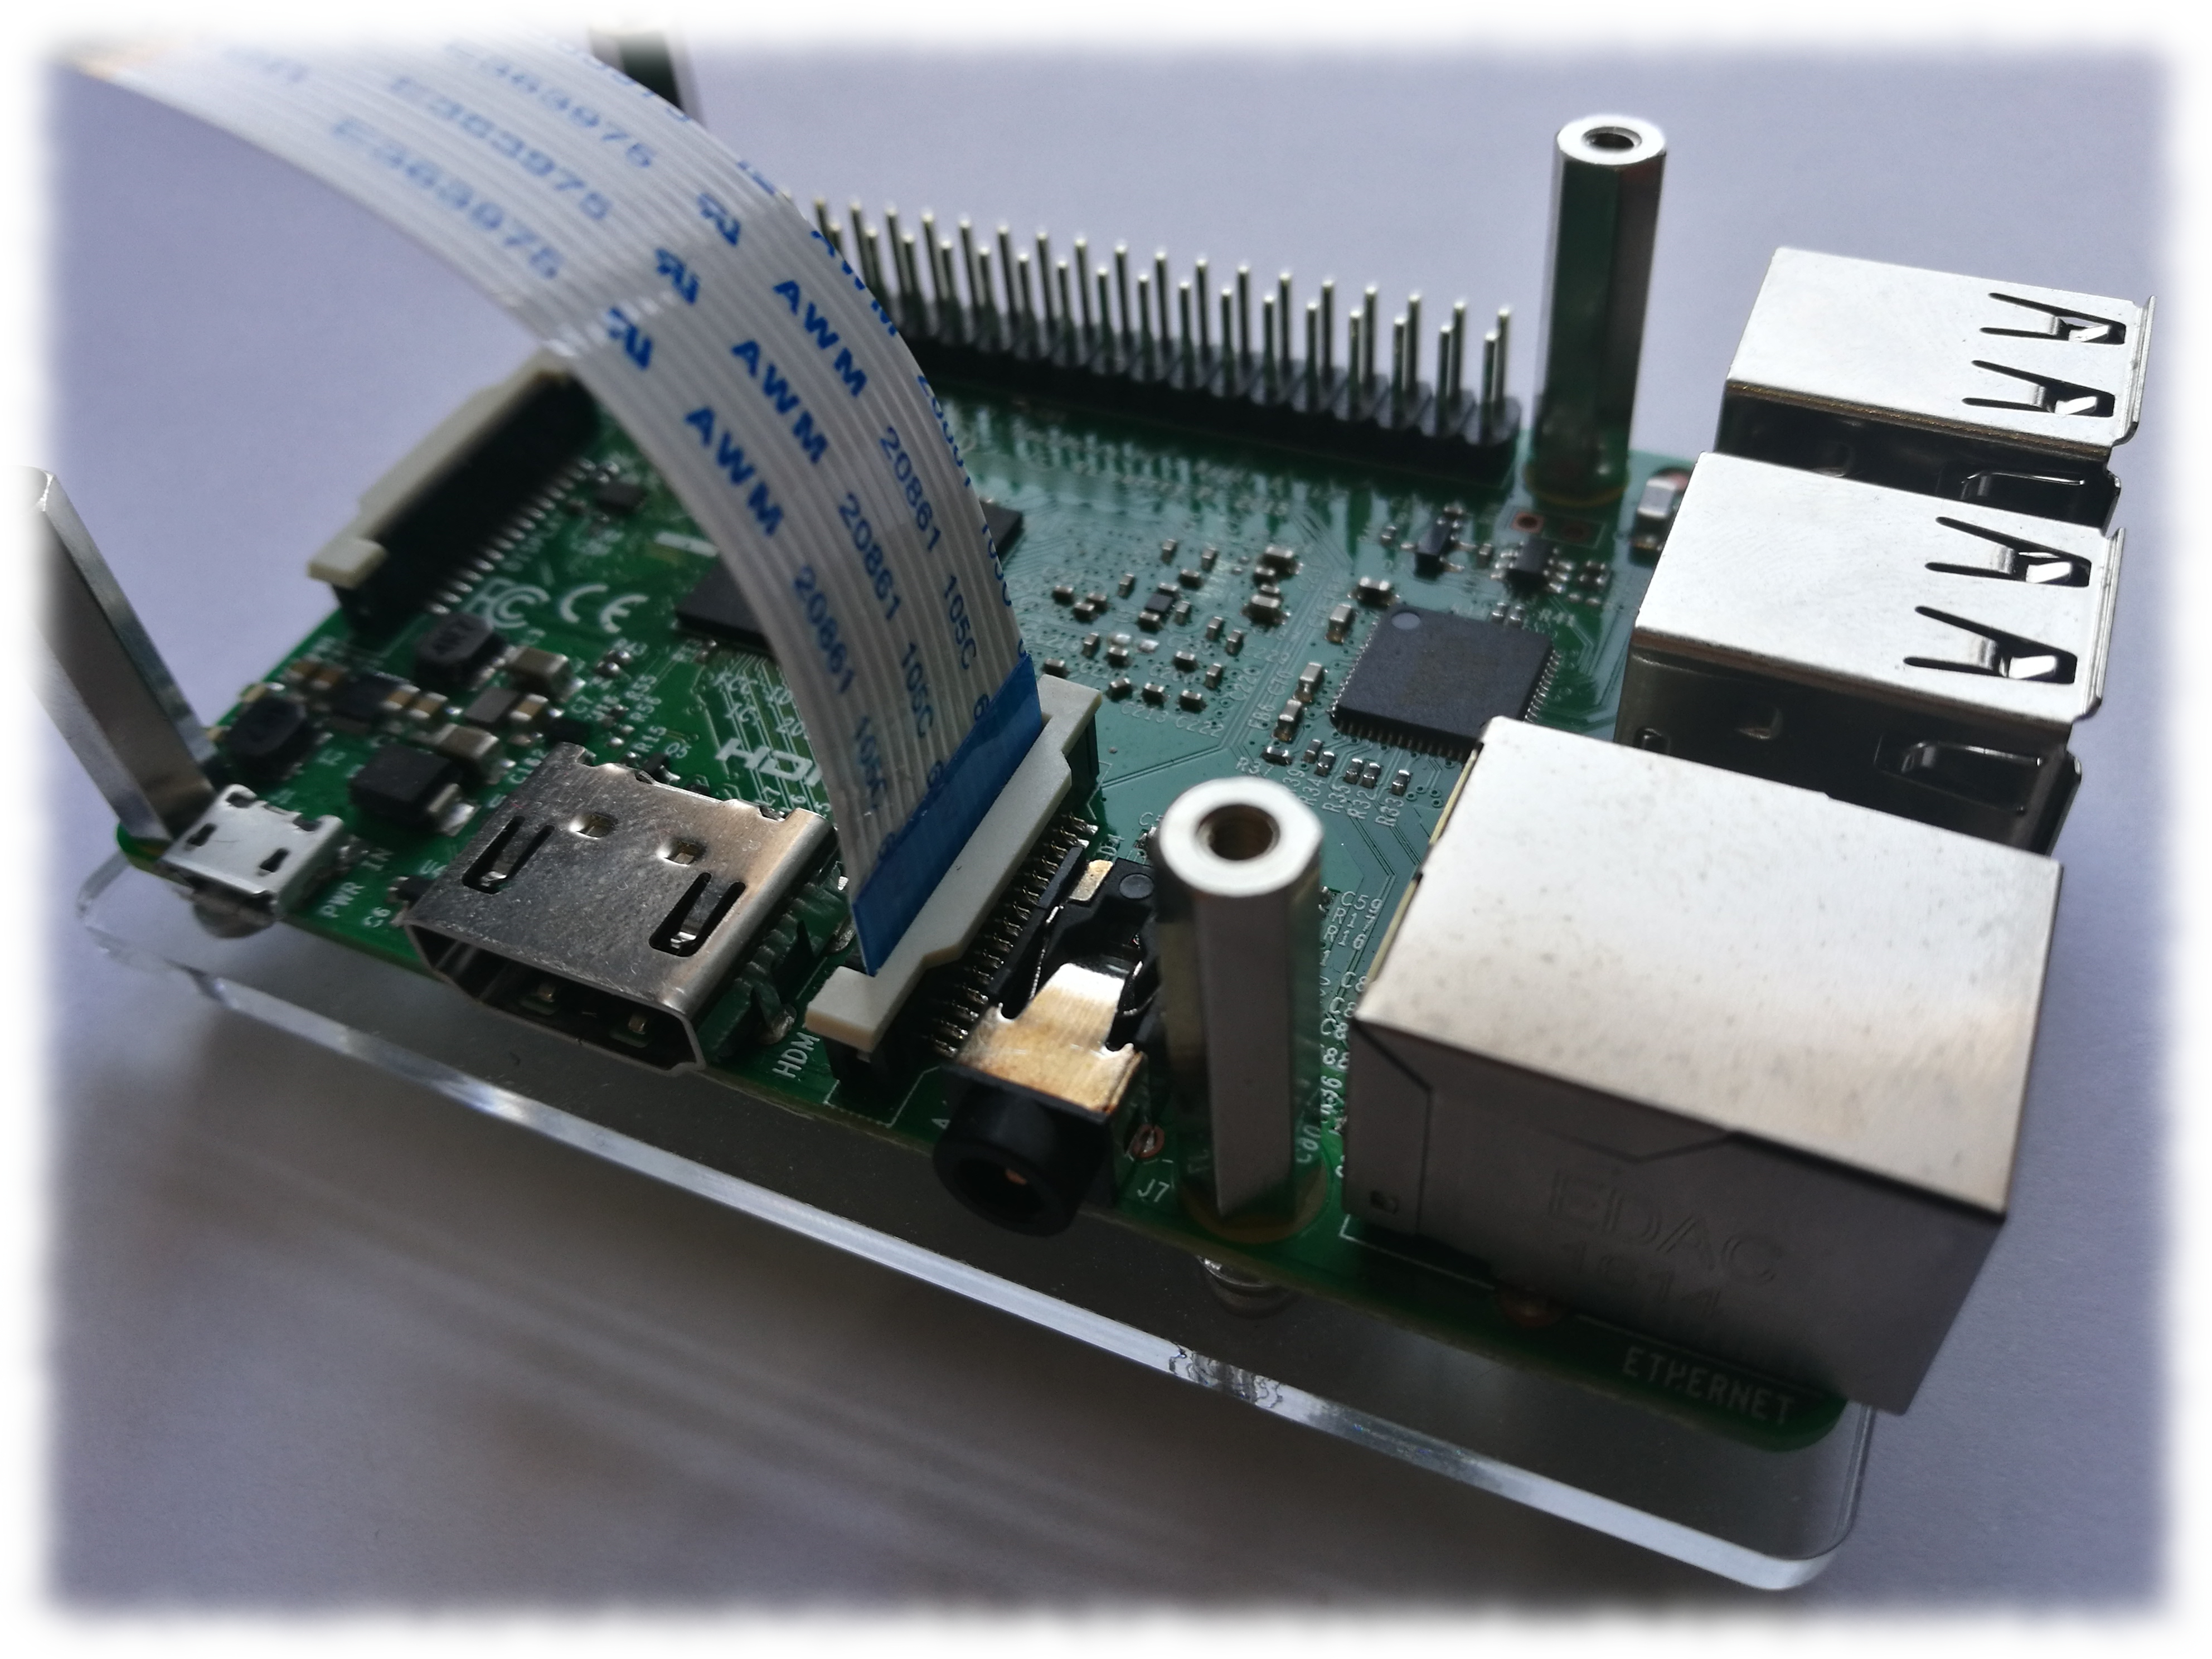
\includegraphics[width=0.75\textwidth]{Appendix_camera_conection.jpg}
		\caption{Connection of the camera module to the Raspberry Pi 3.}
		\label{fig:Appendix_camera_conection}
	\end{center}
\end{figure} %TODO: Cambiar imagen ?


\subsection{Installation of the sensors}
\FIXME{To be continued...} %TODO


\subsection{Installation of the necessary libraries}
Some libraries are needed in order to execute the software developed in this \ac{B.Sc.} Thesis. These libraries are:
\begin{enumerate}
	\item NumPy. \cite{NumPy} Is the fundamental package for scientific computing with Python. NumPy can also be used as an efficient multi-dimensional container of generic data. To install it, the next command needs to be executed:
\begin{console}
$ sudo apt-get install python-numpy python3-numpy
\end{console} %$

	\item Matplotlib. \cite{Hun07} Is a library for the generation of graphic from data contained in list or arrays using Python programming language and the NymPy package. It provides a MATLAB-like interface. To install it, the next command needs to be executed:
\begin{console}
$ sudo apt-get install python-matplotlib python3-matplotlib
\end{console} %$

	\item MP4Box. \cite{MP4Box} It can be used for performing many manipulations on multimedia files like AVI, MPG, TS, but mostly on ISO media files (e.g. MP4, 3GP). The justification for using it is that PiCamera generates the video recording in \emph{h265} format. Therefore, this tool will be used to convert videos from \emph{h265} to \emph{mp4}. The installation can be done using:
\begin{console}
$ sudo apt-get install gpac
\end{console} %$
	Once MP4Box has been installed, any video (named \texttt{video.h264}) can be converted from \emph{h265} to \emph{mp4} at 30 \ac{FPS} using:
\begin{console}
$ MP4Box -fps 30 -add video.h264 video.mp4
\end{console} %$


\FIXME{To be continued...} %TODO
\end{enumerate}

When all this steps has been completed, the Raspberry Pi should be prepared for the correct execution of the software developed in this \ac{B.Sc.} Thesis.
